\documentclass[a4paper,12pt]{article}

\usepackage{amsmath,amssymb,amsthm,tikz}
\usetikzlibrary{calc,arrows.meta}
\usepackage[margin=20mm]{geometry}

\begin{document}\thispagestyle{empty}

\begin{center}
\Large C++ Exercise 4: Running time and abstract data types 
\end{center}

\noindent
\textbf{Deadline:} Friday, October 9, 2020 by 23:59 EEST Timezone.\\
\textbf{How to submit:} GitHub\\
\textbf{Grading:} This exercise is worth 2\% of the total grade.

\begin{enumerate}

\item \textbf{Running time.} Find the best-case and worst-case running times for the algorithms below, by analyzing home many times each line is evaluated, in terms of the input size. The input size is $n$, which is the length of the input list $A$.
\begin{enumerate}
\item \text{\sc Bubble-sort}
\[
\begin{array}{r l}
1 & \text{\textbf{for\ }}m = A.length \text{\textbf{\ downto\ }}2 \\
2 & \hspace{.5cm} \text{\textbf{for\ }} i = 1 \text{\textbf{\ to\ }} m-1 \\
3 & \hspace{1cm} \text{\textbf{if\ }} A[i] > A[i+1] \\
4 & \hspace{1.5cm} swap(A[i],A[i+1]) 
\end{array}
\]
\item \text{\sc Better-Bubble-sort}
\[
\begin{array}{r l}
1 & \text{\textbf{for\ }}m = A.length \text{\textbf{\ downto\ }}2 \\
2 & \hspace{.5cm} sorted = true \\
3 & \hspace{.5cm} \text{\textbf{for\ }} i = 1 \text{\textbf{\ to\ }} m-1 \\
4 & \hspace{1cm} \text{\textbf{if\ }} A[i] > A[i+1] \\
5 & \hspace{1.5cm} swap(A[i],A[i+1]) \\
6 & \hspace{1.5cm} sorted = false \\
7 & \hspace{.5cm} \text{\textbf{if\ }}sorted = true \\
8 & \hspace{1cm} \text{\textbf{return}} 
\end{array}
\]
\end{enumerate}

\item \textbf{Abstract data types.} 
\begin{enumerate}
\item Implement the \textit{circular linked list}, an abstract data type where:
\begin{itemize}
\item each node contains its value and a link to the next node
\item the link on the last node points back to the first node.
\end{itemize}
\vspace{10pt}
\[
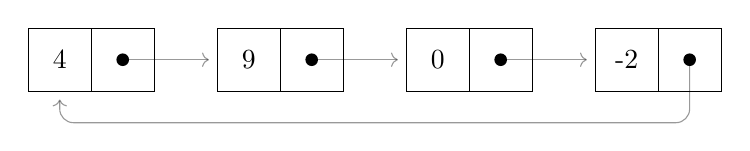
\begin{tikzpicture}[scale=.8,link/.style={opacity=.4,->,shorten >=3pt}]
\draw (0,0) rectangle (2,1); \draw (1,0)--(1,1);
\draw (3,0) rectangle (5,1); \draw (4,0)--(4,1);
\draw (6,0) rectangle (8,1); \draw (7,0)--(7,1);
\draw (9,0) rectangle (11,1); \draw (10,0)--(10,1);
\foreach \x\n in {0/4, 1/9, 2/0, 3/-2}{
  \node at (3*\x+.5,.5) {\n};
  \fill[black] (3*\x+1.5,.5) circle (.1);
}
\draw[link] (1.5,.5)--(3,.5);
\draw[link] (4.5,.5)--(6,.5);
\draw[link] (7.5,.5)--(9,.5);
\draw[link,rounded corners=5pt] (10.5,.5)--++(270:1)--++(180:10)--++(90:.5);
\end{tikzpicture}
\]
\item Implement the \textit{circular linked double list}, an abstract data type where:
\begin{itemize}
\item each node contains its value and links to the nodes below and to the right
\item the link on the last node in each row / column points back to the first node in the row / column
\end{itemize}
You may use the \texttt{vector} STL to implement this abstract data type.
\end{enumerate}
\vspace{10pt}
\[
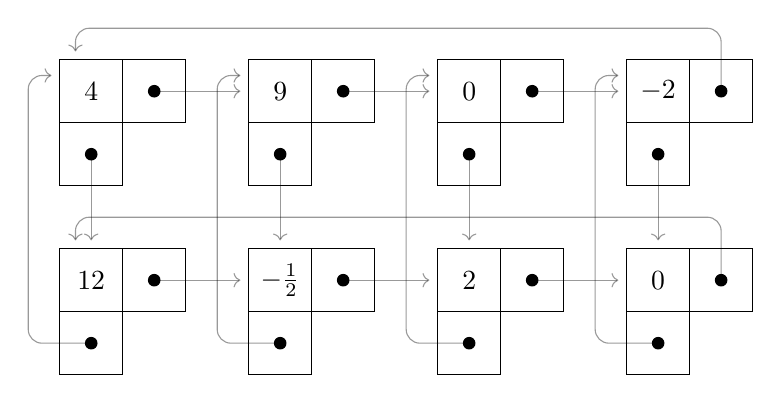
\begin{tikzpicture}[scale=.8,link/.style={opacity=.4,->,shorten >=3pt}]
\foreach \x in {0,1,2,3}{
  \foreach \y in {0,-1}{
    \draw (\x*3,\y*3) rectangle (\x*3+2,\y*3+1);
    \draw (\x*3,\y*3+1) rectangle (\x*3+1,\y*3-1);
  }
}
\foreach \x\y\n in {0/0/4, 1/0/9, 2/0/0, 3/0/-2, 0/-1/12, 1/-1/{-\frac12}, 2/-1/2, 3/-1/0 }{
  \node at (3*\x+.5,\y*3+.5) {$\n$};
  \fill[black] (3*\x+1.5,\y*3+.5) circle (.1);
  \fill[black] (3*\x+.5,\y*3-.5) circle (.1);
}
\foreach \x in {0,1,2}{
  \draw[link] (\x*3+1.5,.5)--(\x*3+3,.5);
  \draw[link] (\x*3+1.5,-2.5)--(\x*3+3,-2.5);
}
\foreach \x in {0,1,2,3}{
  \draw[link] (\x*3+.5,-.5)--(\x*3+.5,-2);
  \draw[link,rounded corners=5pt] (\x*3+.5,-3.5)--++(180:1)--++(90:4.25)--++(0:.5);
}

\draw[link,rounded corners=5pt] (10.5,.5)--++(90:1)--++(180:10.25)--++(270:.5);
\draw[link,rounded corners=5pt] (10.5,-2.5)--++(90:1)--++(180:10.25)--++(270:.5);
\end{tikzpicture}
\]

\end{enumerate}
\end{document}